\documentclass[tikz,border=5mm]{standalone}
\usepackage{amssymb,amsmath,mathtools}
\usetikzlibrary{arrows.meta,decorations.pathreplacing}
\usetikzlibrary{calc,angles,quotes}
\renewcommand{\Re}{\mathrm{Re}}
\renewcommand{\Im}{\mathrm{Im}}

\begin{document}
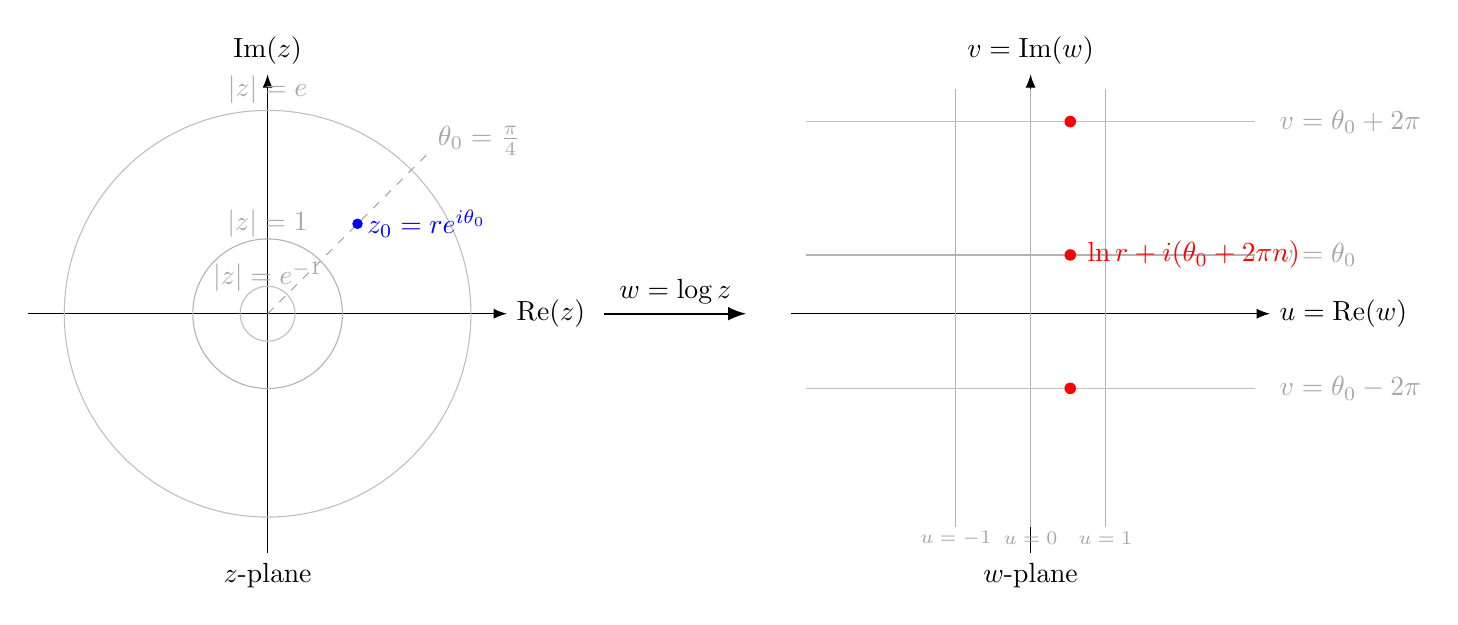
\begin{tikzpicture}[>=Latex,scale=0.95]
%---------------- z-plane (left)
\begin{scope}
% axes
\draw[->] (-3.2,0) -- (3.2,0) node[right] {$\Re(z)$};
\draw[->] (0,-3.2) -- (0,3.2) node[above] {$\Im(z)$};
\node at (0,-3.5) {$z$-plane};
% circles |z| = e^{-1}, 1, e
\draw[gray!50] (0,0) circle (0.3679);   % e^{-1}
\draw[gray!60] (0,0) circle (1.0000);   % 1
\draw[gray!50] (0,0) circle (2.7183);   % e

\node[gray!70] at (0,.5) {$|z|=e^{-1}$};
\node[gray!70] at (0,1.2) {$|z|=1$};
\node[gray!70] at (0,3) {$|z|=e$};

% ray theta = pi/4
\draw[gray!70,dashed] (0,0) -- (2.1213,2.1213); % 3 * (cos45, sin45)
\node[gray!70] at (1.1314*2.5,0.7714*3) {$\theta_0=\frac{\pi}{4}$};

% a sample point z0 = r e^{i theta0}, with r=1.7, theta0=pi/4
\fill[blue] (1.2021,1.2021) circle (2pt) node[anchor=west] {$z_0=re^{i\theta_0}$};

% formula label
%\node[align=left] at (-2.7,-2.6)
%{$\displaystyle \log z=\ln r+i(\theta+2\pi n),\ n\in\mathbb Z$};
\end{scope}
%------------- mapping arrow
\draw[->,thick] (4.5,0) -- (6.4,0) node[midway,above] {$w=\log z$};
%---------------- w-plane (right)
\begin{scope}[xshift=10.2cm]
% axes
\draw[->] (-3.2,0) -- (3.2,0) node[right] {$u=\Re(w)$};
\draw[->] (0,-3.2) -- (0,3.2) node[above] {$v=\Im(w)$};
\node at (0,-3.5) {$w$-plane};

% vertical lines u = ln r for r = e^{-1},1,e
\draw[gray!60] (-1.0000,-2.85) -- (-1.0000,3.0); % ln(e^{-1}) = -1
\draw[gray!60] ( 0.0000,-2.85) -- ( 0.0000,3.0); % ln(1) = 0
\draw[gray!60] ( 1.0000,-2.85) -- ( 1.0000,3.0); % ln(e) = 1
\node[gray!70, font=\scriptsize] at (-1.00, -3) {$u=-1$};
\node[gray!70, font=\scriptsize] at ( 0.00, -3) {$u=0$};
\node[gray!70, font=\scriptsize] at ( 1.00, -3) {$u=1$};

% horizontal lines v = theta0 + 2*pi*n for n=-1,0,1, with theta0=pi/4
\draw[gray!50] (-3.0,-5.4978+4.5) -- (3.0,-5.4978+4.5); % pi/4 - 2pi
\draw[gray!60] (-3.0, 0.7854) -- (3.0, 0.7854); % pi/4
\draw[gray!50] (-3.0, 7.0686-4.5) -- (3.0, 7.0686-4.5); % pi/4 + 2pi
\node[gray!70, right] at (3.2, 0.7854) {$v=\theta_0$};
\node[gray!70, right] at (3.2, 7.0686-4.5) {$v=\theta_0+2\pi$};
\node[gray!70, right] at (3.2,-5.4978+4.5) {$v=\theta_0-2\pi$};

% image points of z0 on every branch:
% choose r=1.7 -> ln r ≈ 0.5306
\fill[red] (0.5306,-5.4978+4.5) circle (2.2pt);
\fill[red] (0.5306, 0.7854) circle (2.2pt);
\fill[red] (0.5306, 7.0686-4.5) circle (2.2pt);
\node[red,anchor=west] at (0.6306,0.7854)
{$\ln r+i(\theta_0+2\pi n)$};

%% mapping hints
%\draw[->,blue!70,bend left=12] (2.6,0.35) to (1.02,0.35);
%\node[blue!70,anchor=west] at (1.10,0.45) {$|z|=r \ \mapsto\ u=\ln r$};
%
%\draw[->,blue!70,bend left=14] (-2.4,2.2) to (-1.0,0.7854);
%\node[blue!70,anchor=west] at (-2.9,2.3)
%{$\theta=\theta_0 \ \mapsto\ v=\theta_0+2\pi n$};
\end{scope}
\end{tikzpicture}
\end{document}